\documentclass[english]{article} 
\usepackage{geometry}
\geometry{hmargin=2.1cm,vmargin=3.5cm}
\usepackage{multicol}
\usepackage{lipsum}
\usepackage{graphicx}
\usepackage[hidelinks]{hyperref}
\usepackage[utf8]{inputenc}
\usepackage{babel}
\usepackage[T1]{fontenc}
\usepackage{textcomp}
\usepackage{lmodern, newunicodechar}
\usepackage{textgreek}
\usepackage{url}
\usepackage{enumitem}
\usepackage{minted}
\usepackage{amsmath}
\usepackage{mathtools}
\usepackage{mathrsfs}
\usepackage{sistyle}
\usepackage{csvsimple}
\usepackage{caption}

\usepackage[backend=bibtex,style=numeric]{biblatex}
\addbibresource{references.bib}


\usepackage{pythonhighlight}


\begin{document}

\begin{titlepage}

\begin{center}
        
\includegraphics[scale=0.05]{rsc/logos/LOGO-UNIV-FC_COULEUR.png}
        \hspace{1cm}
        
\includegraphics[scale=0.025]{rsc/logos/utinam.png}
        \hspace{1cm}
        
\includegraphics[scale=0.04]{rsc/logos/CNRS.png}
        \hspace{1cm}
        
\includegraphics[scale=0.04]{rsc/logos/femto.png}
        \hspace{1cm}
\end{center}

    \vbox{ }

    \vbox{ }

    \begin{center}
        % Øverste del av siden
                
        \textsc{\Large Free Project Techhnical Report - M2 CompuPhys}\\[1cm]

        % \vbox{ }
        % Tittel
        \noindent\makebox[\linewidth]{\rule{.7\paperwidth}{.6pt}}\\[0.7cm]
        { \Huge \bfseries - Technical Report - \\ Implementation of Direct Feedback Alignment Using PyTorch}\\[0.25cm]
        \noindent\makebox[\linewidth]{\rule{.7\paperwidth}{.6pt}}\\[0.7cm]
        \LARGE{Léo BECHET}\\
        \small{University of Franche-Comté}\\[1.2cm]
        
        \vfill
        % Forfatter
        \large
        % \emph{Skrevet av:}\\[1mm]
        \Large{Under the supervision of Pr.Daniel BRUNNER,\\
        and Dr.Anas SKALLI from the FEMTO-ST Institute}

        % Nederste del av siden
    \end{center}
\end{titlepage}

\newpage
\tableofcontents
% DO THE DEMOS RUN TUTORIAL
% SAY WHIC DEPENDENCIIES TO INSTALL
\newpage

% Mise en page pour l'abstract
\section*{\centering \textbf{Abstract}}

\begin{center}
  \hrulefill\\[0.2cm]
  \begin{minipage}{0.9\textwidth}
      \centering
        The following projects aims to provide a basic framework which can be used to train Artificial Neural Networks using Direct Feedback Alignment. We use the popular PyTorch package to provide a robust and already well documented base framework. \\
      \textbf{Keywords: Python, PyTorch, Direct Feedback Alignment, Backpropagation, Machine Learning, Neural Network Training.}

  \end{minipage}\\[0.2cm]
  \hrulefill
\end{center}



\section{Introduction}
% - we aim to create a framework used to train PyTorch networks using Direct Feedback Alignment
% - A first proof of concept is created (Alpha) to test and expose our approach of DFA training.
% - the Alpha is interactive, meaning it is in a jupyter notebook and the user can play around with different parts of the algorithm.
% - the alpha is very good to get familiar with the principle and toy around before going in the thick of it and diving in the actual implementation of the framework.
% - secondly we build a framework (Beta) that corresponds to the different approach we had to DFA training, precised in the scientific report.
% - the beta is meant to be used as a framework to start project using DFA.


In this project, we aim to create a framework for training PyTorch networks using Direct Feedback Alignment (DFA). To begin with, we have developed an Alpha version of the framework, which serves as a proof of concept and interactive tool. The Alpha version is designed in a Jupyter notebook format, allowing users to explore different aspects of the algorithm.

Our approach with the Alpha version is to familiarize ourselves with the principles of DFA training using a fixed network size, before diving into the actual implementation of the framework. This initial stage helps us understand the underlying concepts better and enables us to make informed decisions while building the final product.

Following the success of the Alpha version, we have moved on to create a Beta version that adheres to the different approaches outlined in our scientific report. The primary objective of this framework is to provide users with a solid foundation upon which they can build their DFA-based projects.

In conclusion, both the Alpha and Beta versions of our Direct Feedback Alignment framework are crucial steps towards empowering users to train PyTorch networks using DFA.



\section{Alpha Version : Proof Of Concept}
% - presented as a Jupyter notebook
% - each part is sepaarate and named
% - we first import dependencies
% '''
% import torch
% import copy
% import torch.nn as nn
% from torch.utils.data import TensorDataset, DataLoader
% import torch.nn.functional as F
% import numpy as np
% from scipy.special import expit
% '''

% - we define a simple torch ANN model and its forward pass
% '''
% class DynamicModel(nn.Module):
%     def __init__(self, layer_sizes, act_function):
%         super(DynamicModel, self).__init__()
%         # Define layers using ModuleList
%         self.layers = nn.ModuleList(
%             [nn.Linear(layer_sizes[i], layer_sizes[i+1]) for i in range(len(layer_sizes) - 1)]
%         )
%         self.act_function = act_function  # Activation function

%     def forward(self, x):
%         # Forward pass through each layer
%         for i, layer in enumerate(self.layers):
%             x = layer(x)
%             # Apply activation to all except the last layer
%             if i < len(self.layers) - 1:
%                 x = self.act_function(x)
%         return x
% '''
% - we define a forward pass that also returns internal activations and a backward pass using DFA
% '''

% # Forward pass using PyTorch model
% def forward_pass(model, x):
%     h1 = model.act_function(model.layers[0](x))
%     a1 = model.layers[0](x)
%     a2 = model.layers[1](h1)
%     y_hat = torch.sigmoid(a2)
%     return a1, h1, a2, y_hat

% # DFA backward pass with PyTorch tensors
% def dfa_backward_pass(e, h1, B1, a1, x):
%     dW2 = -torch.matmul(e, h1.T)
%     da1 = torch.matmul(B1, e) * (1 - torch.tanh(a1) ** 2) # tanh derivative
%     dW1 = -torch.matmul(da1, x.T)
%     db1 = -torch.sum(da1, dim=1, keepdim=True)
%     db2 = -torch.sum(e, dim=1, keepdim=True)
%     return dW1, dW2, db1, db2
% '''


% - we define a standard training loop using pytorch and the forward and backward pass we defined above
% '''
% def train_DFA(model, x, y, n_epochs=10, lr=1e-3, batch_size=200, tol=1e-1):
%     x = torch.tensor(x, dtype=torch.float32)
%     y = torch.tensor(y, dtype=torch.float32)

%     # Initialize random feedback matrix
%     B1 = torch.randn(model.layers[0].out_features, model.layers[-1].out_features)

%     dataset = TensorDataset(x, y)
%     dataloader = DataLoader(dataset, batch_size=batch_size, shuffle=True)

%     angles = []
%     te_dfa = []
%     loss_dfa = []

%     for epoch in range(n_epochs):
%         epoch_loss = 0.0
%         train_error = 0

%         for batch_x, batch_y in dataloader:
%             # Forward pass
%             a1, h1, a2, y_hat = forward_pass(model, batch_x)
%             error = y_hat - batch_y
%             preds = torch.argmax(y_hat, dim=1)
%             truth = torch.argmax(batch_y, dim=1)
%             train_error += (preds != truth).sum().item()

%             # Calculate loss
%             loss_on_batch = F.binary_cross_entropy(y_hat, batch_y)
%             epoch_loss += loss_on_batch.item()

%             # DFA backward pass
%             dW1, dW2, db1, db2 = dfa_backward_pass(error.T, h1.T, B1, a1.T, batch_x.T)

%             # Update weights manually
%             with torch.no_grad():
%                 model.layers[0].weight += lr * dW1
%                 model.layers[0].bias += lr * db1.squeeze()
%                 model.layers[1].weight += lr * dW2
%                 model.layers[1].bias += lr * db2.squeeze()

%         training_error = train_error / len(dataset)
%         print(f"Epoch {epoch+1}: Loss = {epoch_loss / len(dataloader):.4f}, Training Error = {training_error:.4f}")

%         prev_training_error = te_dfa[-1] if te_dfa else 0
%         if np.abs(training_error - prev_training_error) <= tol:
%             te_dfa.append(training_error)
%             print(f'Hitting tolerance of {tol} with {np.abs(training_error - prev_training_error)}')
%             break
%         te_dfa.append(training_error)
%         loss_dfa.append(epoch_loss)

%     return te_dfa, loss_dfa, angles
% '''

% - we also define a training loop using PyTorch's builtin Backpropagation, not described here as not relevant for this project.
% - we load the MNIST dataset from keras, prepare out datasets and train the network on it
% '''
% # Dataset stuff 
% # # ======================== MNIST ============================
% from keras.datasets import mnist
% (X_train, y_train), (X_test, y_test) = mnist.load_data()
% X_train = X_train.astype(np.float32)
% X_test = X_test.astype(np.float32)
% X_train /= 255.0
% X_test /= 255.0
% X_train = X_train.reshape(60000, 28 * 28)
% X_test = X_test.reshape(10000, 28 * 28)
% nb_classes = 10
% y_train = np.eye(nb_classes)[y_train]
% y_test = np.eye(nb_classes)[y_test]
% # # ======================== MNIST ============================

% # Define the model
% input_size = 784 #784
% hidden_size = 200 #800
% output_size = 10 #10
% epochs = 80
% batch_size = 200
% learning_rate = 1e-4
% act_function = nn.Tanh()

% model_DFA = DynamicModel([input_size, hidden_size, output_size], act_function)
% model_BACK = copy.deepcopy(model_DFA)

% # Train the model using DFA
% te_dfa, loss_dfa, angles = train_DFA(model_DFA, X_train, y_train, n_epochs=epochs, lr=learning_rate, batch_size=batch_size, tol = -1)

% # Train using Backprop
% # error with the loss on this one /shrug
% te_back, loss_back = train_BACK(model_BACK, X_train, y_train, n_epochs=epochs, lr=learning_rate, batch_size=batch_size, tol=-1)
% '''
% - we plot the training errors, include figure rsc/alpha/TE.png, training errors show the expected behavior by going down.

% - we test the network on a test dataset and extract valuable informations using confusion matrices, accuracies, recalls and precisions. include figure in rsc/alpha/precs_recalls.png, we spot that for our case, which is a vanilla an unoptimized DFA and backprop, performance are the same with around a 97% accuracy on all digits. DFA looks more consistent tho.



This section presents the proof-of-concept implementation of our approach using a Jupyter notebook. Each component of the implementation is modular and partly-documented. We start by importing the required dependencies for the project. These include libraries such as \texttt{torch} for deep learning, \texttt{numpy} for numerical computations, and \texttt{scipy.special} for activation functions. The imports are as follows:

\begin{python}
import torch
import copy
import torch.nn as nn
from torch.utils.data import TensorDataset, DataLoader
import torch.nn.functional as F
import numpy as np
from scipy.special import expit
\end{python}

We define a simple artificial neural network (ANN) model using PyTorch, with flexibility to specify the layer sizes and activation function. The model's forward pass propagates input through each layer while applying the activation function to all but the last layer. The implementation is as follows:

\begin{python}
class DynamicModel(nn.Module):
    def __init__(self, layer_sizes, act_function):
        super(DynamicModel, self).__init__()
        self.layers = nn.ModuleList(
            [nn.Linear(layer_sizes[i], layer_sizes[i+1]) for i in range(len(layer_sizes) - 1)]
        )
        self.act_function = act_function

    def forward(self, x):
        for i, layer in enumerate(self.layers):
            x = layer(x)
            if i < len(self.layers) - 1:
                x = self.act_function(x)
        return x
\end{python}

To extend functionality, we define a forward pass that outputs intermediate activations in addition to the final predictions. This is crucial for implementing a Direct Feedback Alignment (DFA) backward pass. The forward pass returns the intermediate activations \(a_1, h_1, a_2\), and predictions \(y_{\text{hat}}\). lease note that we hardcoded the return values. This is due to the fact that we will only use 1 hidden layer in this example. 

\begin{python}
def forward_pass(model, x):
    h1 = model.act_function(model.layers[0](x))
    a1 = model.layers[0](x)
    a2 = model.layers[1](h1)
    y_hat = torch.sigmoid(a2)
    return a1, h1, a2, y_hat
\end{python}

The DFA backward pass computes weight updates using a random feedback matrix and activation derivatives. This avoids reliance on backpropagation by propagating the error directly through the feedback paths. Again, please note that weights and bias updates are hardcoded for a 1 hidden layer network.

\begin{python}
def dfa_backward_pass(e, h1, B1, a1, x):
    dW2 = -torch.matmul(e, h1.T)
    da1 = torch.matmul(B1, e) * (1 - torch.tanh(a1)**2)
    dW1 = -torch.matmul(da1, x.T)
    db1 = -torch.sum(da1, dim=1, keepdim=True)
    db2 = -torch.sum(e, dim=1, keepdim=True)
    return dW1, dW2, db1, db2
\end{python}

A custom training loop was implemented for training the model using DFA. The loop involves calculating loss, performing the forward pass, and manually updating weights based on the gradients computed through DFA. Random feedback matrices are initialized for DFA computation. Training error and loss are monitored across epochs. Early stopping is triggered based on a tolerance parameter to ensure computational efficiency:

\begin{python}
def train_DFA(model, x, y, n_epochs=10, lr=1e-3, batch_size=200, tol=1e-1):
    # Initialization and dataset setup
    ...
    for epoch in range(n_epochs):
        for batch_x, batch_y in dataloader:
            # Forward pass
            a1, h1, a2, y_hat = forward_pass(model, batch_x)
            error = y_hat - batch_y

            # Compute gradients and update weights
            dW1, dW2, db1, db2 = dfa_backward_pass(error.T, h1.T, B1, a1.T, batch_x.T)
            with torch.no_grad():
                model.layers[0].weight += lr * dW1
                model.layers[0].bias += lr * db1.squeeze()
                model.layers[1].weight += lr * dW2
                model.layers[1].bias += lr * db2.squeeze()
        ...
\end{python}

To evaluate the proof of concept, the MNIST dataset is loaded and preprocessed. Input features are normalized, and labels are one encoded for classification. The model architecture includes 784 input neurons ($28\times28$ input images loaded linearly), 200 hidden neurons in 1 layer, and 10 output neurons(0-9 digits). We trained two models: one using DFA and another using standard backpropagation. Both models were trained for 80 epochs with a batch size of 200 and a learning rate of \(10^{-4}\).

\begin{python}
# Load and preprocess MNIST
from keras.datasets import mnist
(X_train, y_train), (X_test, y_test) = mnist.load_data()
...
y_train = np.eye(nb_classes)[y_train]
y_test = np.eye(nb_classes)[y_test]
\end{python}

Finally, training errors for both models were plotted, revealing the expected behavior of decreasing error rates. Results on the test dataset showed comparable performance for DFA and backpropagation, with around 97\% accuracy across all digits. Confusion matrices, precision, recall, and other metrics confirm that DFA provides consistent results while maintaining the simplicity of its approach. Fig.\ref{fig:alpha_TE} illustrates the training error evolution and performance metrics are displayed in Fig.\ref{fig:alpha_precs_rec}. 

\begin{figure}[h!]
  \centering
  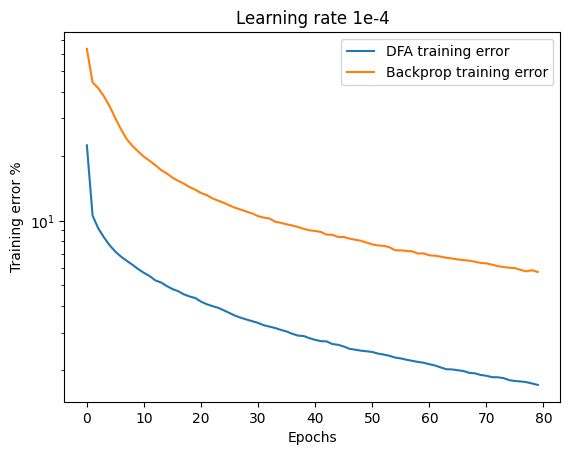
\includegraphics[width=0.48\textwidth]{rsc/alpha/TE.png}
  \caption{Training error on an example run}\label{fig:alpha_TE}
\end{figure}

\begin{figure}[H]
  \centering
  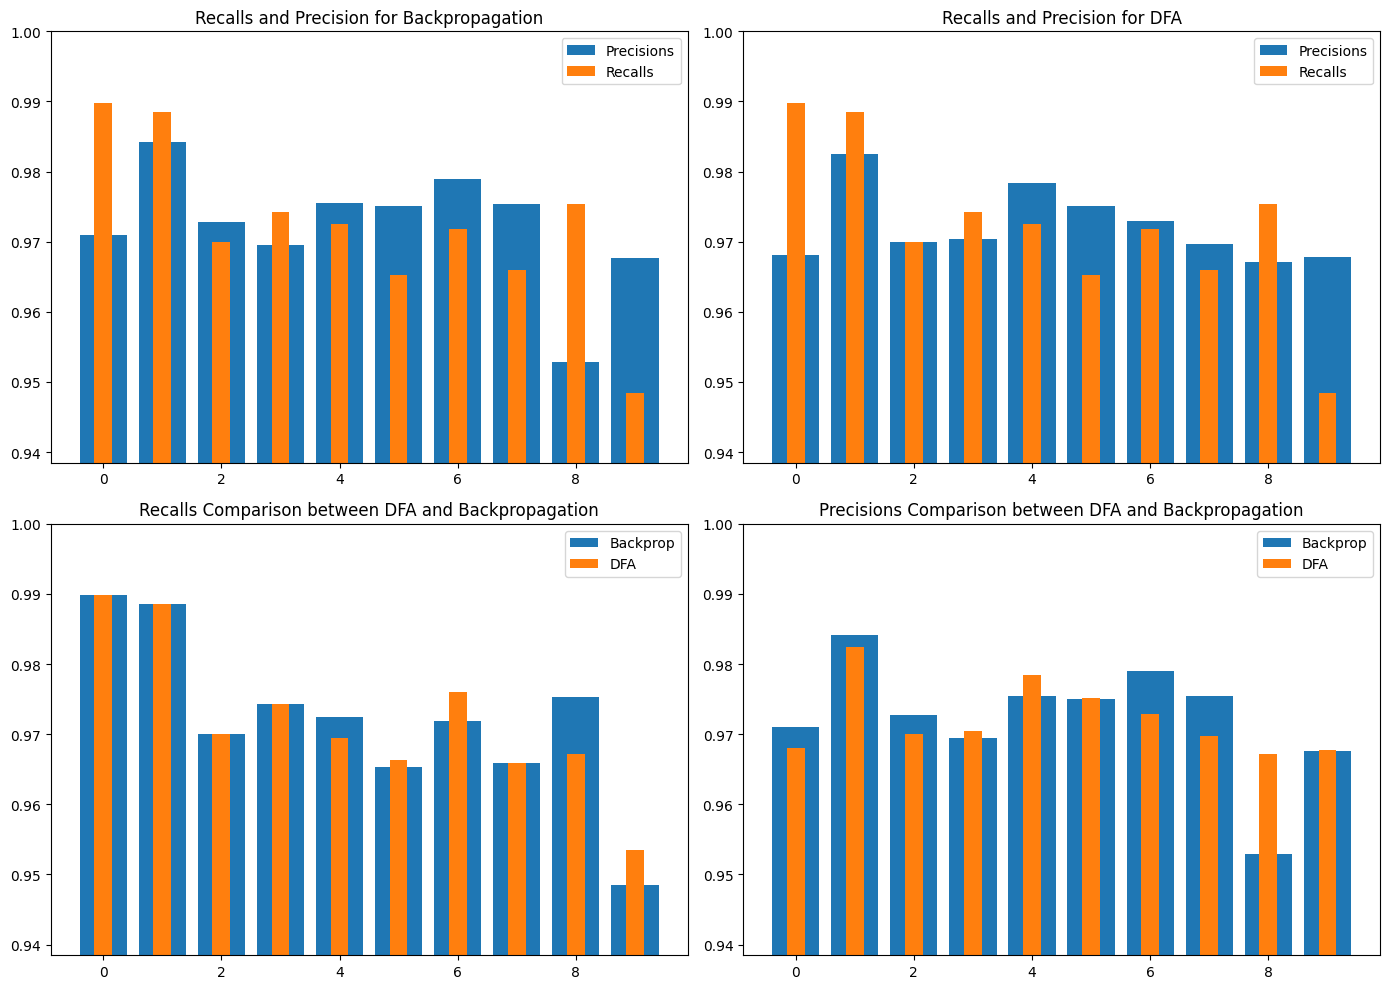
\includegraphics[width=0.8\textwidth]{rsc/alpha/precs_recalls.png}
  \caption{Precisions and recalls comparisons on an example run}\label{fig:alpha_precs_rec}
\end{figure}

We spot that for an example test case, which is a vanilla and unoptimized DFA and backprop, performance are the same with around a 97\% accuracy on all digits. DFA looks more consistent though. We can conclude that this test validates our proof of concept, meaning that DFA works as expected by having equivalent performance to Backpropagation. Please note the difference in scales in Fig.\ref{fig:alpha_TE} which comes from the difference in how this value is estimated.




\section{Beta Version: Framework}



\subsection{User guide}
A Jupyter Notebook which goal is to introduce the worflow of the framework is provided in this project. The code follows a simple example trained on MNIST. Network model creation, including input, hidden layers and output sizes, as well as usage of the training loops, is covered. And boiler-plate testing code is also provided.

Please check the \texttt{framework\_tutorial} for more informations.



\subsection{Model Class}

% \subsubsection{Initialisation}
%     % def __init__(self, layer_sizes, act_function, act_function_derivative, output_function=torch.sigmoid):
%     %     super(DynamicModel, self).__init__()
%     %     # Define layers using ModuleList
%     %     self.layers = nn.ModuleList(
%     %         [nn.Linear(layer_sizes[i], layer_sizes[i+1]) for i in range(len(layer_sizes) - 1)]
%     %     )
%     %     self.layer_sizes = layer_sizes
%     %     self.act_function = act_function  # Activation function
%     %     self.act_function_derivative = act_function_derivative
%     %     self.output_function = output_function

% \subsubsection{Forward passes}

% - describe both forward pass
% - how one doesn't saves hidden activations when just used, but the other does for training

% % # Forward pass using PyTorch model
% % def forward_pass_train(self, x):

% %     a = []
% %     h = [x]
% %     for l_index in range(len(self.layers)-1):
% %         # i-th layer
% %         a.append(self.layers[l_index](h[-1]))
% %         h.append(self.act_function(a[-1]))

% %     # last layer
% %     a_last = self.layers[-1](h[-1])
% %     y_hat = self.output_function(a_last)
% %     return a, h, y_hat #get rid of the x at the start

% % # Forward pass getting rid of a and h list for simple use.
% % def forward(self, x):

% %     a = 0
% %     h = x
% %     for l_index in range(len(self.layers)-1):
% %         # i-th layer
% %         a = self.layers[l_index](h)
% %         h = self.act_function(a)

% %     # last layer
% %     a_last = self.layers[-1](h)
% %     y_hat = self.output_function(a_last)
% %     return y_hat #get rid of the x at the start

% \subsubsection{DFA Backward pass}

% % # DFA backward pass with PyTorch tensors
% % def dfa_backward_pass(self, e, h, a, B): # x is h0 actually

% %     dW = []
% %     db = []

% %     for i in range(len(B)):
% %         da = torch.matmul(B[i], e) * self.act_function_derivative(a[i])
% %         dW.append(-torch.matmul(da, h[i].T))
% %         db.append(-torch.sum(da, dim=1, keepdim=True))

% %     dW.append(-torch.matmul(e, h[-1].T))
% %     db.append(-torch.sum(e, dim=1, keepdim=True))

% %     return dW, db

% \subsubsection{Printing a summary of the model}

% % def summary(self, input_shape):
% % print("===========================MODEL SUMMARY==============================")
% % print(f"{'Layer':<10}{'Input Shape':<20}{'Output Shape':<20}{'Activation':<20}")
% % print("=" * 70)

% % x = torch.rand(*input_shape)  # Dummy input to trace the shapes
% % for i, layer in enumerate(self.layers):
% %     input_shape = x.shape
% %     x = layer(x)  # Forward pass through the layer
% %     output_shape = x.shape
% %     activation = type(self.act_function) if i < len(self.layers) - 1 else type(self.output_function)
% %     activation = str(activation)
% %     print(f"{i:<10}{str(list(input_shape)):<20}{str(list(output_shape)):<20}{activation:<20}")
% % print("=" * 70)
% % print(f'input size  : {self.layer_sizes[0]}')
% % print(f'output size : {self.layer_sizes[-1]}')
% % print(f'layers sizes: {self.layer_sizes}')
% % print("============================END SUMMARY===============================")


\subsubsection{Initialization}

The initialization of the \texttt{DynamicModel} class defines the structure and essential components of the model. The constructor takes the following inputs:

\begin{itemize}
    \item \texttt{layer\_sizes}: A list of integers specifying the number of neurons in each layer, including input, hidden, and output layers.
    \item \texttt{act\_function}: The activation function to be applied between layers (e.g., \texttt{torch.nn.Tanh()}).
    \item \texttt{act\_function\_derivative}: The derivative of the activation function for gradient computations in the DFA backward pass.
    \item \texttt{output\_function}: A function applied to the output layer (default is \texttt{torch.sigmoid}).
\end{itemize}

The code initializes a list of linear layers using \texttt{torch.nn.ModuleList}, which ensures that all layers are properly registered as part of the model. Additionally, the activation and output functions are stored as attributes for use in forward passes.

\begin{python}
def __init__(self, layer_sizes, act_function, act_function_derivative, output_function=torch.sigmoid):
    super(DynamicModel, self).__init__()
    self.layers = nn.ModuleList(
        [nn.Linear(layer_sizes[i], layer_sizes[i+1]) for i in range(len(layer_sizes) - 1)]
    )
    self.layer_sizes = layer_sizes
    self.act_function = act_function
    self.act_function_derivative = act_function_derivative
    self.output_function = output_function
\end{python}

\textbf{Output}: An instance of \texttt{DynamicModel}, ready to perform forward and backward passes.

\subsubsection{Forward Passes}

Two types of forward passes are implemented: one for simple use (without saving intermediate activations) and another for training, where intermediate activations are saved.

The training forward pass, \texttt{forward\_pass\_train}, propagates the input through the model, saving pre-activation values (\(a\)) and post-activation values (\(h\)) for every layer:

\begin{itemize}
    \item \texttt{x}: The input tensor (\(h_0\)) to the network.
    \item \texttt{a}: A list of pre-activation values for each layer.
    \item \texttt{h}: A list of post-activation values for each layer.
    \item \texttt{y\_hat}: The output predictions after applying the output function.
\end{itemize}

\begin{python}
def forward_pass_train(self, x):
    a = []
    h = [x]
    for l_index in range(len(self.layers)-1):
        a.append(self.layers[l_index](h[-1]))
        h.append(self.act_function(a[-1]))

    a_last = self.layers[-1](h[-1])
    y_hat = self.output_function(a_last)
    return a, h, y_hat
\end{python}

The lighter forward pass is used when intermediate activations are not needed. Only the final predictions are returned:

\begin{itemize}
    \item \texttt{x}: The input tensor.
    \item \texttt{y\_hat}: The output predictions.
\end{itemize}

\begin{python}
def forward(self, x):
    a = 0
    h = x
    for l_index in range(len(self.layers)-1):
        a = self.layers[l_index](h)
        h = self.act_function(a)

    a_last = self.layers[-1](h)
    y_hat = self.output_function(a_last)
    return y_hat
\end{python}

\textbf{Output}: In the training pass, intermediate values (\(a\), \(h\)) and predictions (\(y_{\text{hat}}\)) are returned. In the simpler pass, only predictions (\(y_{\text{hat}}\)) are returned.

\subsubsection{DFA Backward Pass}

The backward pass computes weight and bias updates using Direct Feedback Alignment, relying on random feedback matrices (\(B\)). It calculates gradients for each layer using the error (\(e\)), intermediate activations (\(h\)), and pre-activations (\(a\)).

Inputs:
\begin{itemize}
    \item \texttt{e}: Error tensor from the output layer.
    \item \texttt{h}: List of post-activation values for all layers, including the input.
    \item \texttt{a}: List of pre-activation values for all layers.
    \item \texttt{B}: A list of random feedback matrices for each layer.
\end{itemize}

Outputs:
\begin{itemize}
    \item \texttt{dW}: A list of weight gradients for all layers.
    \item \texttt{db}: A list of bias gradients for all layers.
\end{itemize}

The computation involves the algorithm described in the scientific report, section 3.

\begin{python}
def dfa_backward_pass(self, e, h, a, B):
    dW = []
    db = []

    for i in range(len(B)):
        da = torch.matmul(B[i], e) * self.act_function_derivative(a[i])
        dW.append(-torch.matmul(da, h[i].T))
        db.append(-torch.sum(da, dim=1, keepdim=True))

    dW.append(-torch.matmul(e, h[-1].T))
    db.append(-torch.sum(e, dim=1, keepdim=True))

    return dW, db
\end{python}

\subsubsection{Printing a Summary of the Model}

The \texttt{summary} method provides a detailed overview of the model's architecture, including layer indices, input and output shapes, and the activation functions used.

\begin{itemize}
    \item \texttt{input\_shape}: A tuple specifying the shape of the input tensor.
\end{itemize}

The method uses a dummy input tensor to trace the input and output shapes of each layer during a forward pass. For each layer, it prints the layer index, input shape, output shape, and activation type.

\begin{python}
def summary(self, input_shape):
    print("===========================MODEL SUMMARY==============================")
    print(f"{'Layer':<10}{'Input Shape':<20}{'Output Shape':<20}{'Activation':<20}")
    print("=" * 70)

    x = torch.rand(*input_shape)  # Dummy input to trace the shapes
    for i, layer in enumerate(self.layers):
        input_shape = x.shape
        x = layer(x)
        output_shape = x.shape
        activation = type(self.act_function) if i < len(self.layers) - 1 else type(self.output_function)
        activation = str(activation)
        print(f"{i:<10}{str(list(input_shape)):<20}{str(list(output_shape)):<20}{activation:<20}")
    print("=" * 70)
    print(f'input size  : {self.layer_sizes[0]}')
    print(f'output size : {self.layer_sizes[-1]}')
    print(f'layers sizes: {self.layer_sizes}')
    print("============================END SUMMARY===============================")
\end{python}

\textbf{Output}: A printed table summarizing the structure of the model, including layer-wise details and input/output sizes.












\subsection{Training loops}

\subsubsection{Basic training loop}
% - basic training loop using DFA
% - signature is train_basic(model, x, y, n_epochs=10, lr=1e-3, batch_size=200, tol=1e-1, error_function=MNIST_error):

The provided training loop implements Direct Feedback Alignment (DFA) in PyTorch for training a neural network. DFA replaces the standard backpropagation method by using random feedback matrices to compute gradients. Below is a detailed breakdown of each step in the code:

\paragraph{Inputs:}
\begin{itemize}
    \item \texttt{model}: A PyTorch model that implements \texttt{forward\_pass\_train} and \texttt{dfa\_backward\_pass}.
    \item \texttt{x, y}: Training data and labels. Both are converted to PyTorch tensors.
    \item \texttt{n\_epochs}: Number of training epochs.
    \item \texttt{lr}: Learning rate for gradient updates.
    \item \texttt{batch\_size}: Number of samples per batch.
    \item \texttt{tol}: Convergence tolerance based on changes in training error.
    \item \texttt{error\_function}: Function to compute error and misclassification rate (e.g., \texttt{MNIST\_error}).
\end{itemize}

\paragraph{Random Feedback Matrices Initialization}:
\begin{python}
B = [matrix_transfo(torch.empty(layer.out_features, 
     model.layers[-1].out_features).normal_(mean=0,std=1.9)) for layer in model.layers[:-1]]
\end{python}
A list of random matrices (\(B\)) is generated for each layer except the output layer. The \texttt{matrix\_transfo} function can optionally apply transformations to these matrices. We tried using them to skew the value distribution, without good results.

\paragraph{Dataset Preparation}:
The \texttt{TensorDataset} combines inputs (\texttt{x}) and targets (\texttt{y}) into a single dataset, while the \texttt{DataLoader} enables batch-wise data loading with shuffling to improve generalization.

\paragraph{Metrics Initialization}:
\begin{python}
te_dfa = []
loss_dfa = []
\end{python}
Two lists are initialized to record the training error (\texttt{te\_dfa}) and loss (\texttt{loss\_dfa}) for each epoch.

\paragraph{Epoch Loop:}
The outer loop iterates over the specified number of epochs (\texttt{n\_epochs}). Within each epoch, the following steps are executed:

\subparagraph{Batch Loop:}
The \texttt{DataLoader} provides batches of data (\texttt{batch\_x} and \texttt{batch\_y}), iterating through the entire dataset. This part can be linked to the scientific report, section 3.

\begin{itemize}
    \item \textbf{Forward Pass:}
    The model's \texttt{forward\_pass\_train} method computes:
    \begin{itemize}
        \item Pre-activation values (\(a\)) for each layer (list).
        \item Post-activation values (\(h\)), including the input (\(h_0 = x\)) (list).
        \item Predictions (\(y_{\text{hat}}\)) after applying the output function(list).

    \end{itemize}

    \item \textbf{Error Computation:}
    The error signal is computed as:
    \[
    \text{error} = y_{\text{hat}} - \text{batch\_y}
    \]
    The \texttt{error\_function} also calculates the number of misclassified samples and updates the cumulative training error.
    Since MNIST is used throughout this project, we use the following function to compute the errorr and training error.:
    \begin{python}
def MNIST_error(y_hat, batch_y, train_error):
    error = y_hat - batch_y
    preds = torch.argmax(y_hat, dim=1)
    truth = torch.argmax(batch_y, dim=1)
    train_error += (preds != truth).sum().item()

    return error, train_error
    \end{python}

    \item \textbf{Loss Calculation:}
    The binary cross-entropy loss between predictions (\(y_{\text{hat}}\)) and ground truth labels (\(\text{batch\_y}\)) is computed:
    \[
    \text{Loss}_{\text{batch}} = \texttt{F.binary\_cross\_entropy}(y_{\text{hat}}, \text{batch\_y})
    \]

    BCELoss is chosen here as it is standard for classificattion tasks.

    \item \textbf{Transpose Activations:}
    To ensure compatibility with feedback matrices, pre-activation (\(a\)) and post-activation (\(h\)) tensors are transposed (\(a^T\) and \(h^T\)).

    \item \textbf{DFA Backward Pass:}
    Using the \texttt{dfa\_backward\_pass} method, the weight gradients (\(dW\)) and bias gradients (\(db\)) are computed. Please check scientific report, section 3, for further informations.

    \item \textbf{Manual Weight Updates:}
    Model weights and biases are updated manually using the computed gradients and learning rate (\(\eta\)):
    \[
    W_i \leftarrow W_i + \eta dW_i, \quad b_i \leftarrow b_i + \eta db_i
    \]
\end{itemize}

\paragraph{Epoch Metrics and Convergence Check:}
The total epoch loss (\texttt{epoch\_loss}) and training error (\texttt{training\_error}) are recorded. If the change in training error falls below the specified tolerance (\texttt{tol}), training terminates early.

\begin{python}
if np.abs(training_error - prev_training_error) <= tol:
    print(f'Hitting tolerance of {tol} with {np.abs(training_error - prev_training_error)}')
    break
\end{python}

\paragraph{Output:}
The function returns two lists:
\begin{itemize}
    \item \texttt{te\_dfa}: Training error for each epoch.
    \item \texttt{loss\_dfa}: Loss for each epoch.
\end{itemize}
The results can be used for further analysis or plotting.






\subsubsection{Batch-averaged training loop}
% - same as the basic training loop except we perform an average on the input and output of the batch, we update only once per batch instead of Ntimes
% -signature is train_averaged(model, x, y, n_epochs=10, lr=1e-3, batch_size=200, tol=1e-1)


In this modified version of the training loop, the inputs, activations, pre-activations, and outputs are averaged across the batch to compute a "master error." This approach differs from the previous loop by aggregating batch-level information into a single representative value, which is then used for error computation and gradient updates. Below is a detailed explanation of the changes:

\paragraph{Relevant Code for Averaging:}
The following lines have been added to the batch loop:
\begin{python}
for i in range(len(a)):
    a[i] = torch.mean(a[i], dim=0).unsqueeze(0)

for i in range(len(h)):
    h[i] = torch.mean(h[i], dim=0).unsqueeze(0)

y_hat = torch.mean(y_hat, dim=0).unsqueeze(0)
batch_y = torch.mean(batch_y, dim=0).unsqueeze(0)
batch_x = torch.mean(batch_x, dim=0).unsqueeze(0)

# Recompute error using averaged batches
error = y_hat - batch_y
\end{python}

\paragraph{Changes Compared to the Original Loop:}
\begin{itemize}
    \item \textbf{Averaging Pre-Activations (\(a\)) and Activations (\(h\)):}
    The pre-activations (\(a\)) and activations (\(h\)) are averaged across the batch along the first dimension (\texttt{dim=0}). Each resulting tensor is reshaped into a single-row tensor using \texttt{unsqueeze(0)}.

    \item \textbf{Averaging Outputs (\(y_{\text{hat}}\)) and Ground Truth (\(\text{batch\_y}\)):}
    The predicted outputs (\(y_{\text{hat}}\)) and ground truth labels (\(\text{batch\_y}\)) are also averaged along the batch dimension to produce a single representative prediction and target.

    \item \textbf{Averaging Inputs (\(\text{batch\_x}\)):}
    Similarly, the batch inputs (\(\text{batch\_x}\)) are averaged to obtain a single representative input vector for the entire batch.

    \item \textbf{Recomputing Error:}
    After averaging, the error is recomputed as:
    \[
    \text{error} = y_{\text{hat}} - \text{batch\_y}
    \]
    This averaged error serves as the "master error" for Direct Feedback Alignment.

\end{itemize}







\subsubsection{Per class batch-averaged training loop}
% - same as above but instead we average per class 
% - signature is MNIST_train_class_averaged(model, x, y, n_epochs=10, lr=1e-3, batch_size=200, tol=1e-1, classes=10):


This modified batch loop introduces class-wise averaging for inputs, activations, pre-activations, and outputs within each batch. The primary goal is to compute class-level representations and update the model based on these averaged values, rather than individual sample-level gradients. Below, the differences from the previous loop are explained.

\paragraph{Class-Wise Indexing}:
\begin{python}
class_indices = [ [] for _ in range(classes)]
for item in range(len(batch_y)):
    class_indices[np.argmax(batch_y[item])].append(item)
\end{python}
This section initializes a list of indices for each class (\texttt{class\_indices}). For every sample in the batch, the class corresponding to its encoded label (\texttt{batch\_y}) is determined using \texttt{np.argmax}, and the sample's index is added to the appropriate class list. 

\paragraph{Class-Wise Averaging}:
\begin{python}
for indices in class_indices:
    if indices == []:
        continue

    subset_a = []
    subset_h = []

    for i in range(len(a)):
        subset_a.append(torch.mean(a[i][indices], dim=0).unsqueeze(0))

    for i in range(len(h)):
        subset_h.append(torch.mean(h[i][indices], dim=0).unsqueeze(0))

    sub_y_hat = torch.mean(y_hat[indices], dim=0).unsqueeze(0)
    sub_batch_y = torch.mean(batch_y[indices], dim=0).unsqueeze(0)
\end{python}
This loop processes each class separately:
\begin{itemize}
    \item If no samples belong to a class (\texttt{indices == []}), the loop skips to the next class.
    \item For each layer, pre-activations (\(a\)) and post-activations (\(h\)) of the samples in the class are averaged along the batch dimension (\texttt{dim=0}). The averaged tensors are unsqueezed to retain the correct shape for subsequent computations.
    \item Similarly, predictions (\(y_{\text{hat}}\)) and ground truth labels (\(\text{batch\_y}\)) are averaged over the class's samples.
\end{itemize}

\paragraph{Recomputed Error Signal}:
\begin{python}
error = sub_y_hat - sub_batch_y
\end{python}
The error is recomputed based on the class-wise averaged predictions and labels. This replaces the sample-level error from the previous loop.

\paragraph{Key Differences from the Previous Loop:}
\begin{itemize}
    \item \textbf{Class-Averaging:} 
    Unlike the previous loop, where computations were performed on individual samples, this loop averages inputs, activations, and outputs over all samples belonging to the same class within a batch.
    \item \textbf{Reduced Gradient Updates:}
    Gradient updates are performed at the class level, reducing the frequency of updates compared to the sample-wise approach.
    \item \textbf{Improved Stability:}
    By aggregating information at the class level, the updates are expected to be less noisy, potentially improving the training stability and convergence.
    \item \textbf{Error Signal Recalculation:}
    The error is recalculated using class-averaged predictions and labels, ensuring consistency with the aggregated representations.
\end{itemize}

\paragraph{Benefits of the New Approach:}
Class-wise averaging reduces the variability in gradient computations caused by individual samples. This can lead to more robust updates, especially in scenarios with imbalanced or noisy data. Additionally, this method aligns the training process with the objective of minimizing class-level errors rather than individual sample errors. The behavior of this approach ought to be studied separately from this project alone, as it could lead to interesting result.







% % Should I even put that: answer is no.
% \subsubsection{Per class batch-averaged with learning rate scheduler training loop}
% % - same as above but learning rate is determined in function of the epoch number
% % - signature is MNIST_train_class_averaged_LR_scheduler(model, x, y, lr_schedule, n_epochs=10, batch_size=200, tol=1e-1, classes=10)



\section{How to use the provided demos}

\paragraph{Notebooks} Notebooks can be run as is, granted that dependencies are present and well configured on the host machine. In case of issues, please check the error messages as it most likely will be a missing dependency.

\paragraph{Python Scripts} Python scripts are provided as is as an example. They should however work right out of the box, granted that dependencies are present and well configured on the host machine. While scripts work, we encourage the user to fiddle around the code. Some part have been coomented out and can leave some room for experimentation. We do assume the user to already be familiar with the Technical report content, especially regarding training loop functions' signatures.


\section{Free Project versioning breakdown}

\subsubsection{Alpha}
There are 2 notebooks that answers to the goals set by the Alpha version. The XOR test shows that DFA can be used to solve non-linear problem but do not provide much insight when comparing the DFA and Backpropagation. For this, please look at the MNIST test, which uses a more complex network for digits recognition in an image.
Those 2 notebooks show a basic implementation of DFA, solve 2 simple problems, and compare performances with DFA. Thus it checks all requirements fro the Alpha. More advanced comparison between DFA and Backpropagation can be found in the scientific report.

\subsubsection{Beta}
Due to the nature of the project being focused on research, the goaals of this section shifted during time.
While it was at first planned to analyze more in depth the difference in performance between DFA and Backpropagation, it was decided that it would be more fruitful to analyze a novel approach in training, using averages on batches.
However, please note that while being succintly answered to, the requiremnts of this section have been completed. Scripts found in the Beta files do allow for the comparison of the angles (cf. Section 4.4 for analysis). The behavior difference between DFA and Backpropagation have been studied under the approach of averaging batches. Finally, a framework has been developped to ease the use of DFA in project. This framework was developped alongside the test files.

\subsubsection{Gold}
Gold requirements weren't met in any capacity.

% \begin{figure}[H]
%   \begin{center}
%     \includegraphics[scale=0.5]{8_oct_ref_star and sat.png}
%     \caption{Position of the Asteroid and Star During the First Observation on October 8th}
%     \label{origine 8}
%   \end{center}
% \end{figure}


% \begin{equation}
%         C_F^* = r - mag_i^{cal*}
%         \label{CF}
% \end{equation}\\







% \newpage
% \begin{appendix}
% \section{Appendix}



% \end{appendix}


% \bibliography{references} 
% \bibliographystyle{ieeetr}

\end{document}